
\chapter{Laufzeitsicht}

\section{Szenario I}
\textbf{Auswählen eines Roboters}\\

\begin{figure}[h]
    \centering
    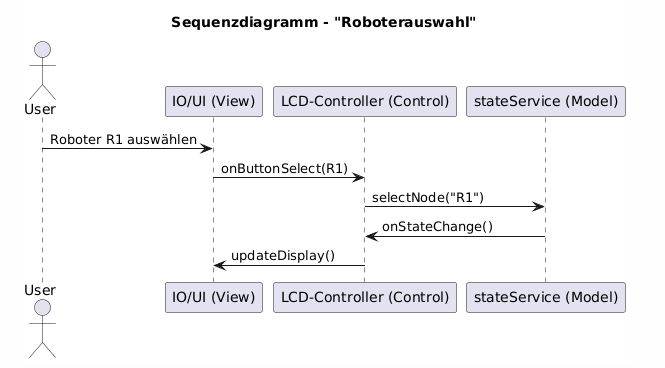
\includegraphics[width=0.8\linewidth]{diagrams/roboterAuswahl_250525.png}
    \caption{Auswahl des Roboters}
    \label{fig:Auswahl}
\end{figure}

\clearpage
\section{Szenario II}
\textbf{Bewegungsbefehl über GUI}\\

\begin{figure}[h]  
    \centering
    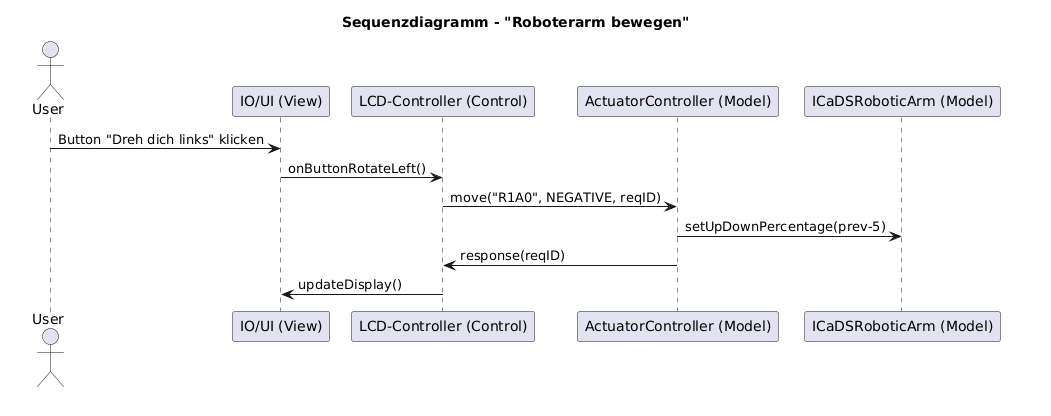
\includegraphics[width=0.8\linewidth]{diagrams/moveBefehl_250525.png}
    \caption{Bewegungsbefehl über GUI}
    \label{fig:Bewegungsbefehl}
\end{figure}

%\clearpage
%\section{Szenario III}
%\textbf{Fehlerfall: Verbindung zu Roboter fällt aus}\\

%\begin{figure}[h]  
%    \centering
%    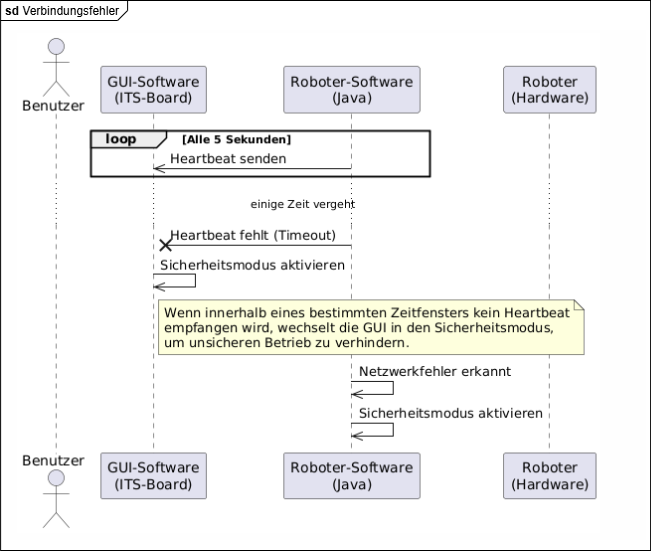
\includegraphics[width=0.8\linewidth]{diagrams/Verbindungsverlust.png}
%    \caption{Verbindungsverlust}
%    \label{fig:Verbindungsverlust}
%\end{figure}



